% This is the Reed College LaTeX thesis template. Most of the work
% for the document class was done by Sam Noble (SN), as well as this
% template. Later comments etc. by Ben Salzberg (BTS). Additional
% restructuring and APA support by Jess Youngberg (JY).
% Your comments and suggestions are more than welcome; please email
% them to cus@reed.edu
%
% See http://web.reed.edu/cis/help/latex.html for help. There are a
% great bunch of help pages there, with notes on
% getting started, bibtex, etc. Go there and read it if you're not
% already familiar with LaTeX.
%
% Any line that starts with a percent symbol is a comment.
% They won't show up in the document, and are useful for notes
% to yourself and explaining commands.
% Commenting also removes a line from the document;
% very handy for troubleshooting problems. -BTS

% As far as I know, this follows the requirements laid out in
% the 2002-2003 Senior Handbook. Ask a librarian to check the
% document before binding. -SN

%%
%% Preamble
%%
% \documentclass{<something>} must begin each LaTeX document
\documentclass[12pt,twoside]{reedthesis}
% Packages are extensions to the basic LaTeX functions. Whatever you
% want to typeset, there is probably a package out there for it.
% Chemistry (chemtex), screenplays, you name it.
% Check out CTAN to see: http://www.ctan.org/
%%
\usepackage{graphicx,latexsym}
\usepackage{amsmath}
\usepackage{amssymb,amsthm}
\usepackage{longtable,booktabs,setspace}
\usepackage{chemarr} %% Useful for one reaction arrow, useless if you're not a chem major
\usepackage[hyphens]{url}
% Added by CII
\usepackage{hyperref}
\usepackage{lmodern}
\usepackage{float}
\floatplacement{figure}{H}
% End of CII addition
\usepackage{rotating}

\usepackage[utf8]{inputenc}
\usepackage[spanish]{babel}
% Next line commented out by CII
%%% \usepackage{natbib}
% Comment out the natbib line above and uncomment the following two lines to use the new
% biblatex-chicago style, for Chicago A. Also make some changes at the end where the
% bibliography is included.
%\usepackage{biblatex-chicago}
%\bibliography{thesis}


% Added by CII (Thanks, Hadley!)
% Use ref for internal links
\renewcommand{\hyperref}[2][???]{\autoref{#1}}
\def\chapterautorefname{Chapter}
\def\sectionautorefname{Section}
\def\subsectionautorefname{Subsection}
% End of CII addition

% Added by CII
\usepackage{caption}
\captionsetup{width=5in}
% End of CII addition

% \usepackage{times} % other fonts are available like times, bookman, charter, palatino

% Syntax highlighting #22
  \usepackage{color}
  \usepackage{fancyvrb}
  \newcommand{\VerbBar}{|}
  \newcommand{\VERB}{\Verb[commandchars=\\\{\}]}
  \DefineVerbatimEnvironment{Highlighting}{Verbatim}{commandchars=\\\{\}}
  % Add ',fontsize=\small' for more characters per line
  \usepackage{framed}
  \definecolor{shadecolor}{RGB}{248,248,248}
  \newenvironment{Shaded}{\begin{snugshade}}{\end{snugshade}}
  \newcommand{\AlertTok}[1]{\textcolor[rgb]{0.94,0.16,0.16}{#1}}
  \newcommand{\AnnotationTok}[1]{\textcolor[rgb]{0.56,0.35,0.01}{\textbf{\textit{#1}}}}
  \newcommand{\AttributeTok}[1]{\textcolor[rgb]{0.77,0.63,0.00}{#1}}
  \newcommand{\BaseNTok}[1]{\textcolor[rgb]{0.00,0.00,0.81}{#1}}
  \newcommand{\BuiltInTok}[1]{#1}
  \newcommand{\CharTok}[1]{\textcolor[rgb]{0.31,0.60,0.02}{#1}}
  \newcommand{\CommentTok}[1]{\textcolor[rgb]{0.56,0.35,0.01}{\textit{#1}}}
  \newcommand{\CommentVarTok}[1]{\textcolor[rgb]{0.56,0.35,0.01}{\textbf{\textit{#1}}}}
  \newcommand{\ConstantTok}[1]{\textcolor[rgb]{0.00,0.00,0.00}{#1}}
  \newcommand{\ControlFlowTok}[1]{\textcolor[rgb]{0.13,0.29,0.53}{\textbf{#1}}}
  \newcommand{\DataTypeTok}[1]{\textcolor[rgb]{0.13,0.29,0.53}{#1}}
  \newcommand{\DecValTok}[1]{\textcolor[rgb]{0.00,0.00,0.81}{#1}}
  \newcommand{\DocumentationTok}[1]{\textcolor[rgb]{0.56,0.35,0.01}{\textbf{\textit{#1}}}}
  \newcommand{\ErrorTok}[1]{\textcolor[rgb]{0.64,0.00,0.00}{\textbf{#1}}}
  \newcommand{\ExtensionTok}[1]{#1}
  \newcommand{\FloatTok}[1]{\textcolor[rgb]{0.00,0.00,0.81}{#1}}
  \newcommand{\FunctionTok}[1]{\textcolor[rgb]{0.00,0.00,0.00}{#1}}
  \newcommand{\ImportTok}[1]{#1}
  \newcommand{\InformationTok}[1]{\textcolor[rgb]{0.56,0.35,0.01}{\textbf{\textit{#1}}}}
  \newcommand{\KeywordTok}[1]{\textcolor[rgb]{0.13,0.29,0.53}{\textbf{#1}}}
  \newcommand{\NormalTok}[1]{#1}
  \newcommand{\OperatorTok}[1]{\textcolor[rgb]{0.81,0.36,0.00}{\textbf{#1}}}
  \newcommand{\OtherTok}[1]{\textcolor[rgb]{0.56,0.35,0.01}{#1}}
  \newcommand{\PreprocessorTok}[1]{\textcolor[rgb]{0.56,0.35,0.01}{\textit{#1}}}
  \newcommand{\RegionMarkerTok}[1]{#1}
  \newcommand{\SpecialCharTok}[1]{\textcolor[rgb]{0.00,0.00,0.00}{#1}}
  \newcommand{\SpecialStringTok}[1]{\textcolor[rgb]{0.31,0.60,0.02}{#1}}
  \newcommand{\StringTok}[1]{\textcolor[rgb]{0.31,0.60,0.02}{#1}}
  \newcommand{\VariableTok}[1]{\textcolor[rgb]{0.00,0.00,0.00}{#1}}
  \newcommand{\VerbatimStringTok}[1]{\textcolor[rgb]{0.31,0.60,0.02}{#1}}
  \newcommand{\WarningTok}[1]{\textcolor[rgb]{0.56,0.35,0.01}{\textbf{\textit{#1}}}}

% To pass between YAML and LaTeX the dollar signs are added by CII
\title{}
\author{}
% The month and year that you submit your FINAL draft TO THE LIBRARY (May or December)
\date{}
\division{}
\advisor{}
\institution{}
\degree{}
%If you have two advisors for some reason, you can use the following
% Uncommented out by CII
% End of CII addition

%%% Remember to use the correct department!
\department{}
% if you're writing a thesis in an interdisciplinary major,
% uncomment the line below and change the text as appropriate.
% check the Senior Handbook if unsure.
%\thedivisionof{The Established Interdisciplinary Committee for}
% if you want the approval page to say "Approved for the Committee",
% uncomment the next line
%\approvedforthe{Committee}

% Added by CII
%%% Copied from knitr
%% maxwidth is the original width if it's less than linewidth
%% otherwise use linewidth (to make sure the graphics do not exceed the margin)
\makeatletter
\def\maxwidth{ %
  \ifdim\Gin@nat@width>\linewidth
    \linewidth
  \else
    \Gin@nat@width
  \fi
}
\makeatother

\renewcommand{\contentsname}{Table of Contents}
% End of CII addition

\setlength{\parskip}{0pt}

% Added by CII
  %\setlength{\parskip}{\baselineskip}
  \usepackage[parfill]{parskip}

\providecommand{\tightlist}{%
  \setlength{\itemsep}{0pt}\setlength{\parskip}{0pt}}

\Acknowledgements{
I want to thank a few people.
}

\Dedication{
You can have a dedication here if you wish.
}

\Preface{
This is an example of a thesis setup to use the reed thesis document class
(for LaTeX) and the R bookdown package, in general.
}

\Abstract{
The preface pretty much says it all.

\par

Second paragraph of abstract starts here.
}

% End of CII addition
%%
%% End Preamble
%%
%
\begin{document}

% Everything below added by CII

\frontmatter % this stuff will be roman-numbered
\pagestyle{empty} % this removes page numbers from the frontmatter
  \begin{acknowledgements}
    I want to thank a few people.
  \end{acknowledgements}
  \begin{preface}
    This is an example of a thesis setup to use the reed thesis document class
    (for LaTeX) and the R bookdown package, in general.
  \end{preface}
  \hypersetup{linkcolor=black}
  \setcounter{tocdepth}{2}
  \tableofcontents

  \listoftables

  \listoffigures
  \begin{abstract}
    The preface pretty much says it all.
    
    \par
    
    Second paragraph of abstract starts here.
  \end{abstract}
  \begin{dedication}
    You can have a dedication here if you wish.
  \end{dedication}
\mainmatter % here the regular arabic numbering starts
\pagestyle{fancyplain} % turns page numbering back on

\hypertarget{introduccion}{%
\chapter*{Introducción}\label{introduccion}}
\addcontentsline{toc}{chapter}{Introducción}

\hypertarget{rmd-basics}{%
\chapter{Planteamiento de la necesidad}\label{rmd-basics}}

\hypertarget{planteamiento-del-problema}{%
\section{Planteamiento del problema}\label{planteamiento-del-problema}}

Los centros de datos son una parte esencial para las empresas, ya que es donde reside el equipo de telecomunicaciones, almacenamiento y procesamiento de datos críticos para un negocio.
Lo cual, facilita la toma de decisiones.
Adicionalmente un centro de datos debe tener por lo menos un cuarto separado, donde se encuentre el suministro de energía independiente y control de clima Corp (2011).

Esto con el propósito de \ldots{}

El consumo de energía eléctrica dentro de un centro de datos es de alrededor de 45\% por el equipo de tecnologías de la información, en otras palabras, servidores y equipo de telecomunicaciones; el 55\% es consumida por las instalaciones, donde se incluye sistema de distribución, fuentes de alimentación ininterrumpidas, sistemas de enfriamiento Geng (2014).

Las tecnologías de la información juegan una parte vital dentro de una empresa. Ya qué, estas tecnologías son utilizadas para ejecutar procesos críticos de una empresa, por lo tanto, es necesario mantener su óptima operación.
Por esta razón, es necesario monitorear cada aspecto

Pero, en caso de que sí se dañase algún componente y se requiera reemplazo, ya sea: disco duro, fuente de poder, memoria RAM, etc. En algunas ocasiones, para realizar este reemplazo es necesario crear una ventana de mantenimiento; puede tardarse días o meses dependiendo del nivel de criticidad de los procesos que se estén ejecutando.

Existen periodos de tiempo donde no se esta utilizando al máximo el equipo de cómputo. Lo cual es un sobre aprovisionamiento de recursos de cómputo. Un estudio realizado en 2012 por \emph{Natural Resources Defense Council}, donde se estimo que en promedio servidores que ejecutan una sola aplicación tienden a utilizar entre 5\% y 15\% de poder de cómputo Whitney \& Kennedy (2012)
Por otra parte, se estima que en grandes centros de datos el porcentaje de servidores obsoletos se encuentra entre 20\% y 30\% Delforge (2014).

Por el contrario, si una empresa está teniendo un crecimiento bastante acelerado donde la capacidad de cómputo con la que cuentan actualmente será insuficiente en poco tiempo. La empresa se verá en la necesidad de adquirir nuevo equipo de cómputo. El tiempo de entrega dependerá del lugar de entrega y disponibilidad del equipo en cuestión Dell (2015). Lo cual, puede generar problemas al no tener la infraestructura necesaria para escalar el servicio, lo que conlleva a una posibilidad de pérdida de clientes e inestabilidad de los servicios.

\hypertarget{condiciones-a-considerar-cuando-se-quiere-migrar-a-la-nube}{%
\section{Condiciones a considerar cuando se quiere migrar a la nube}\label{condiciones-a-considerar-cuando-se-quiere-migrar-a-la-nube}}

Existen varias considerados que se deben tomar en cuenta cuando se esta decidiendo que tipo de modelo de la nube es el mejor para la empresa. Para esto, es necesario determinar cuales son los requisitos que se debe de cumplir la empresa:
\begin{itemize}
\tightlist
\item
  Requisitos o regulaciones a cumplir. Estas serán las que dictaminen que modelo de despliegue se utilizará.
\item
  Recursos financieros disponibles a invertir.
\item
  Locación geográfica. Esto es importante ya que dependiendo de la ubicación de los clientes puede variar la latencia. Por esto, es importante saber donde se encuentran los centros de datos de los proveedores de nube.
\item
  Elasticidad y demanda
\item
  Contratos, gastos de capital y de operación.
\end{itemize}
\hypertarget{desarrollo-o-introduccion-sobre-el-orden-de-migracion.}{%
\subsection{Desarrollo o introducción sobre el orden de migración.}\label{desarrollo-o-introduccion-sobre-el-orden-de-migracion.}}

Un problema que pueden enfrentar las nuevas empresas, es la adopción del cómputo en la nube, ya que, ya no se encuentra en su etapa de adopción. Por lo que es necesario adoptarla lo mas pronto posible, para poder competir en el mercado tecnológico.

Los beneficios económicos obtenidos al migrar a la nube también están ligados a sacrificios computacionales, entre estos están:
\begin{itemize}
\tightlist
\item
  perdida de control sobre los sistemas.
\item
  aplicaciones comparten recursos.
\item
  latencia sobre peticiones es dictaminada por los recursos disponibles en ese momento.
\end{itemize}
Estos recursos incluyen:
- ciclos de CPU
- datos en memoria
- datos en cache
- datos en dispositivos de almacenamiento.

\hypertarget{cuando-es-recomendable-cambiarse-a-la-nube}{%
\subsection{Cuando es recomendable cambiarse a la nube}\label{cuando-es-recomendable-cambiarse-a-la-nube}}

Cuando los servicios no requieren un alto rendimiento tiene sentido virtualizar esos sistemas, ya que pueden ser fáciles de pausar y reiniciar sin que las aplicaciones sepan que se movieron de centro de datos.

El problema con arquitecturas virtualizadas aparece cuando las aplicaciones tienen alta demanda en almacenamiento y conectividad. Un disco virtualizado tratada de reportar el numero de \emph{IOS}(Operaciones por segundo), pero el hardware que esta usando es compartido, y es difícil mantener la consistencia de esta operación.

\hypertarget{objetivo-general}{%
\section{Objetivo General}\label{objetivo-general}}

Crear un esquema para migración de infraestructura física de TI a la nube, con el fin de agilizar y reducir el proceso de migración que necesita realizar el usuario.

\hypertarget{objetivos-especificos}{%
\subsection{Objetivos específicos}\label{objetivos-especificos}}
\begin{itemize}
\item
  Crear un modelo del dominio del proceso de migración utilizando diseño basado en dominio (\emph{Domain Driven Design})
\item
  Desarrollar un esquema en base al modelo conceptual
\item
  Utilizar tecnologías de orquestación, microservicios y contenedores para la implementación del esquema.
\item
  Desarrollar una aplicación la cual implementará el esquema de migración y utilizará las tecnologías antes mencionadas.
\end{itemize}
\hypertarget{justificacion}{%
\section{Justificación}\label{justificacion}}

El cómputo en la nube ha transformado como las tecnologías de información ofrecen sus servicios y, además, como son consumidas Pinkelman (1993). Las compañías que arriendan su infraestructura o servicios de cómputo son conocidos como proveedores de nube. Actualmente, existen múltiples proveedores de nube alrededor del mundo. Esto les da la oportunidad a las empresas de adquirir los servicios de los proveedores, lo cual podría expandir sus mercados a uno global. Estos servicios son presentados en un catálogo, en donde un usuario u organización puede seleccionar el servicio deseado, utilizarlo y al final solo pagar por el tiempo de consumo, como un pago más de utilidades. Esto les da a los usuarios la posibilidad de acceder a un gran poder de cómputo sin necesidad de una fuerte inversión inicial. Por lo que brinda a las empresas grandes facilidades, ya que no solo reduce el costo de inversión inicial. Además, permite administrar el equipo de cómputo desde un solo lugar. Un ejemplo claro de esto, es el caso del Hospital Firmley Park donde se necesitaba reducir el tiempo administrativo del equipo de cómputo. La solución a este problema fue virtualizar las computadoras de escritorio de los empleados, con el objetivo de poder administrar todo desde un solo lugar, y se accedía a estas utilizando conexión remota (``Frimley,'' 2018).

Gracias al cómputo en la nube es posible tener múltiples respaldos de aplicaciones o computadoras, no solo en diferentes computadoras, sino hasta en diferentes países. Por esta razón, es posible brindar un mejor rendimiento a los clientes, dado que es posible tener instancias de una aplicación lo más cercano posible a él.

La migración de tecnologías de la información a la nube en muchas ocasiones requiere de una gran planeación de la empresa, ya que existen múltiples factores que se deben de considerar. Adicionalmente, si no se tiene el conocimiento ni las herramientas para realizarlo puede resultar en una gran problemática. Un ejemplo de esto es no tomar en consideración los procesos que utilicen equipo \emph{legacy} para algunas aplicaciones cruciales de la empresa Zou \& Kontogiannis (2000) . El problema radica en que quizás la aplicación no interactúe correctamente la aplicación con el servidor, y se tenga que adaptar de alguna forma o modificar el código de esta. Lo cual puede generar un retraso o fracaso en la adopción del cómputo en la nube.

Por último, se creará una aplicación que utilice un esquema de detección, replicación y migración a la nube. Esta aplicación realizará lo siguiente: Durante el periodo de detección, buscará el equipo de cómputo dentro de una red, obtendrá información crucial de cada uno de estos (CPU, RAM, disco duro). Esta información se utilizará para crear máquinas virtuales. Durante el periodo de migración, en los equipos de cómputo se iniciará la tarea de creación de imagines virtuales de estos. Estas imágenes se utilizarán para subirlas a la nube.

\hypertarget{ref_labels}{%
\chapter{Marco Teórico}\label{ref_labels}}

\hypertarget{virtualizacion}{%
\section{Virtualización}\label{virtualizacion}}

La virtualización es una forma de abstracción donde los componentes de hardware son presentarlos de una forma lógica Kusnetzky (2011), con los cuales, se pueden crear maquinas virtuales.
En otras palabras, la virtualización permite utilizar los recursos físicos de una computadora para crear y alojar \emph{N} cantidad de máquinas virtuales. Para poder realizar estas tareas es necesario un hipervisor. El hipervisor se encarga de administrar los recursos de cómputo y proveerlos a las máquinas virtuales. Existen dos tipos de hipervisores:
\begin{itemize}
\item
  Tipo 1 o \emph{Bare Metal}. Es conocido como nativo, ya que corre encima del hardware de la máquina, como si fuera un sistema operativo, esto permite un aislamiento verdadero entre cada sistema operativo de cada \emph{VM}.
\item
  Tipo 2 o \emph{Hosted}. Se ejecuta por encima del sistema operativo de la maquina anfitrión, esté se encarga de mostrar los recursos disponibles al hipervisor.
\end{itemize}
La ``máquina virtual'' fue desarrollada por \emph{IBM} en los años 60, donde\,se tenía acceso concurrente e interactivo a una computadora central desde varias terminales (monitores remotos). Cada máquina virtual era una réplica representativa de la computadora central; es decir, daba la impresión de estar físicamente en una computadora real Ali \& Meghanathan (2011).~

\hypertarget{computo-en-la-nube}{%
\section{Cómputo en la nube}\label{computo-en-la-nube}}

El cómputo en la nube es un modelo para el aprovisionamiento de recursos de cómputo, los cuales son presentados en forma de catálogo. En este catálogo se presentan diversos tipos de servicios, tales como: redes, servidores, almacenamiento, aplicaciones, que pueden ser rápidamente aprovisionados y liberados con un esfuerzo mínimo de administración o de interacción con el proveedor de servicios. Adicionalmente, el cómputo en la nube está compuesto principalmente por cinco características esenciales Mell, Grance, \& others (2011).~~

Las principales características del cómputo en la nube son:~
~
\begin{itemize}
\item
  Servicio en demanda. El cliente puede adquirir el poder de cómputo necesario, automáticamente sin necesidad de interacción con el proveedor.~
\item
  Conectividad. Los servicios son disponibles a través de la red, y pueden ser accedidos a través de distintas plataformas.~~
\item
  Aprovisionamiento. El poder de cómputo\,está configurado para servir múltiples clientes en un modelo multi-cliente, con diferentes recursos físicos y virtuales que son asignados y reasignados de acuerdo con la demanda.~
\item
  Elasticidad. El aprovisionamiento puede ser elástico y escalable. En muchos casos puede ser automática, que escale rápidamente ya sea creciendo o disminuyendo dependiendo de la demanda.~
\item
  Servicios medidos. Los recursos del cómputo en la nube son controlados y optimizados utilizando una capacidad métrica, que se puede medir por almacenamiento, procesamiento, ancho de banda o usuarios activos. La utilización de recursos puede ser monitorizada, controlada y reportada. Proveyendo transparencia tanto para el proveedor como el consumidor de sus servicios.~~
  ~
\end{itemize}
Adicionalmente existen múltiples formas de despliegue, las cuales pueden tener diversos usos dependiendo en el ambiente en el que se utiliza. Los modelos de despliegue son:~
\begin{itemize}
\item
  Nube privada. La infraestructura le pertenece a una empresa. Además, la nube puede estar administrada por la empresa dueña o por terceros. A su vez, puede residir dentro o fuera de la empresa.~
\item
  Nube comunitaria. Está constituida por múltiples comunidades u organizaciones las cuales comparten recursos para un fin en común.~
\item
  Nube pública. En este modelo la infraestructura de la nube puede ser provista por organizaciones o empresas para el uso del público y está la pertenece a proveedores de nube.~
\item
  Nube híbrida. Este modelo está compuesto de dos o más modelos.~
\end{itemize}
Uno de los grandes beneficios del modelo de nube privada, es que da, la posibilidad de brindar una buena calidad de servicios, tiempo de respuesta. Para poder implementar este modelo es necesario utilizar un sistema operativo o plataforma, como los son: \emph{Openstack}, \emph{Cloudstack} Foundation (2017), \emph{VMware vCloud} (``Vcloud suite,'' 2018).~\emph{Openstack} es un sistema operativo que controla una gran cantidad de recursos de cómputo, almacenamiento y red Openstack (2015). Los recursos son administrados por medio de un panel de control, el cual, puede ser accedido por un navegador web, donde solo tienen acceso los administradores y los. Por último, \emph{Openstack} es una plataforma de software libre, la cual es la más utilizada por la comunidad de software libre, además, está apoyada por múltiples empresas, entre ellas, \emph{Red Hat}, \emph{HP},\emph{Google}, etc.~

El computo en la nube brinda diferentes niveles de servicios, en donde dependiendo del nivel seleccionado se tendrá más capacidad de personalización. Los principales niveles de servicios IBM (2018) :
\begin{itemize}
\item
  Software as a Service (SaaS). Las aplicaciones basadas en la nube, las cuales son ejecutadas en computadoras distantes ``en la nube'' que pertenecen y son operadas por otros, las cuales conectan las computadoras de los usuarios vía internet y, usualmente, navegador web.
\item
  Platform as a service (PaaS). Provee un ambiente donde todo lo que se requiere para soportar un ciclo de desarrollo e implementación de aplicaciones web, sin la necesidad de comprar o manejar hardware, software.
\item
  Infrastructure as a service (IaaS). Provee a las compañías con recursos computacionales incluyendo servidores, redes, almacenamiento, y espacio dentro de un centro de datos con pago por uso.
\end{itemize}
Los niveles de servicios que ofrece la nube han incrementado la complejidad de los sistemas actuales, lo cual ha aumentado el número de actividades de los administradores de sistemas. Estas actividades suelen ser repetitivas como: crear máquinas virtuales, instalación de actualizaciones, software o dependencias de este, aunque muchas de estas actividades se pueden ser automatizadas utilizando \emph{scripts}. El problema recae en que muchos \emph{scripts} son creados para realizar tareas en un ambiente especifico, además, de que en muchas ocasiones no son documentados apropiadamente, y en algunas ocasiones es necesario tener un cierto nivel de conocimiento en programación, por otro lado, para ejecutar \emph{scripts}, es necesario obtener acceso al servidor donde serán ejecutarlos. Como resultado, ha sido necesario encontrar nuevas formas de realizar estas tareas repetitivas.

\hypertarget{ansible}{%
\subsection{Ansible}\label{ansible}}

En el mercado actual de las tecnologías de la información se ha incrementado la velocidad de desarrollo y mantenimiento.
La unión de las áreas de desarrollo de software y operaciones ha creado una nueva área llamada DevOps Geerling (2015). DevOps utiliza prácticas del desarrollo de software en la administración de infraestructura como código (\emph{Infrastructure-as-code} IaC). \emph{IaC} es un algoritmo que se encarga de instalar dependencias, controladores necesarios por un programa en específico en un servidor Wittig \& Wittig (2016). Por último, DevOps promueve el uso de conjuntos de \emph{scripts}, modelos para automatización y configuración. Esto con el propósito de reutilizar código y mejorar los tiempos de desarrollo e implementación. Existen múltiples herramientas para DevOps tales como:~

• \emph{Puppet} (2017a)~

• \emph{Chef} (2018a)~

• \emph{Ansible} (2017b)

La funcionalidad de estos programas es la administración y orquestación de infraestructura.

\emph{Ansible} solo necesita un nodo de administración, el cual cuenta con un inventario y múltiples \emph{playbook}, estos últimos son los archivos de configuración, implementación y orquestación. Dentro del inventario se crean grupos en, los cuales se agregan los nombres de los servidores o direcciones IPs. Dentro de \emph{playbook} se configuran las tareas a realizar; estos archivos son creados utilizando el formato \emph{YAML}, por otro lado, los módulos utilizan \emph{JSON}. Se utiliza \emph{SSH} para la conectividad remota y no requiere abrir puertos extras.~Adicionalmente, solo requiere tener instalado* \emph{Python}.

\hypertarget{microservicios}{%
\section{Microservicios}\label{microservicios}}

Tradicionalmente, las aplicaciones son programadas en una sola instancia donde todas las actividades residen en una misma aplicación, también conocido como arquitectura monolítica. Lo cual, genera una problemática al tratar de actualizar el código de la aplicación, ya que muchas ocasiones puede contar con cientos si no miles de líneas de código. Además, son difíciles de comprender y mantener. Por otro lado, cuando se requiere escalar una porción de la aplicación es necesario escalar toda la aplicación, lo cual genera un mayor costo. La figura \ref{figura1} se puede ver varios grupos de desarrolladores trabajando en la misma aplicación sin tener definido que partes de la aplicación le pertenecen.
\begin{figure}[h!]
  \centering
  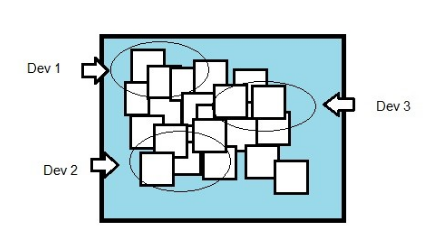
\includegraphics[scale=0.5]{./figure/Cap3/monoFig1.png}
  \caption{Aplicación monolítica}\label{figura1}
\end{figure}
A diferencia de la arquitectura monolítica, la arquitectura orientada a servicios, esta constituida por múltiples servicios, los cuales trabajan en conjunto para realizar una tarea.
El desarrollo orientado a dominio tiene como objetivo desarrollar una aplicación, la cual debe expresar el objetivo de un negocio Adicionalmente, las características. La entrega continua, virtualización, bajo demanda, automatización de infraestructura, sistemas en escala. Estas son las características que ayudan a implementar microservicios Newman (2015). Microservicios es un conjunto de servicios autónomos que trabajan para alcanzar una meta en común. Como se habló con anterioridad las aplicaciones monolíticas limitan la forma de actualizar las aplicaciones ya que se requiere un cierto periodo de tiempo para realizar mantenimiento en el cual se realizan actualizaciones, además, de que limita las actualizaciones de esquemas y formas de manejo de datos. El alcance de cada servicio se enfoca en los alcances del negocio, esto permite reconocer con mayor facilidad el alcance o dominio de cada servicio. Uno de los beneficios que ofrece esta arquitectura es poder utilizar diversas tecnologías ya sea lenguajes de programación, base de datos ya que cada servicio es independiente de otro. Las características claves de los microservicios son:
\begin{itemize}
\tightlist
\item
  Diseño orientado a dómino. Es un enfoque para el desarrollo de software con necesidades complejas mediante una profunda conexión entre la implementación y los conceptos del modelo y núcleo del negocio.
\item
  Principio de responsabilidad simple. De acuerdo con la filosofía de Unix cada servicio es responsable de una parte única de la funcionalidad y lo hace bien Raymond (2003).
\item
  Interfaz explicita
\item
  \emph{DURS independiente (Deploy, Update, Replace, Scale)} Cada servicio se puede implementar, actualizar, reemplazar y escalar de forma independiente.
\item
  \emph{Endpoints/ pipes} Cada microservicio posee su lógica de dominio y se comunica con otros a través de protocolos simples, como REST, el cual provee conectividad.
\end{itemize}
La forma en que se comunican entre sí los servicios es utilizando llamadas a través de la red. Esto puede ser utilizando RPC (Remote Procedure Calls) o REST (REpresentation State Transfer).

Un microservicio puede ser implementado en múltiples ambientes tales como:
\begin{itemize}
\tightlist
\item
  Máquinas virtuales
\item
  Contenedores
\item
  Plataforma como servicio (PaaS)
\end{itemize}
\begin{figure}[h!]
  \centering
  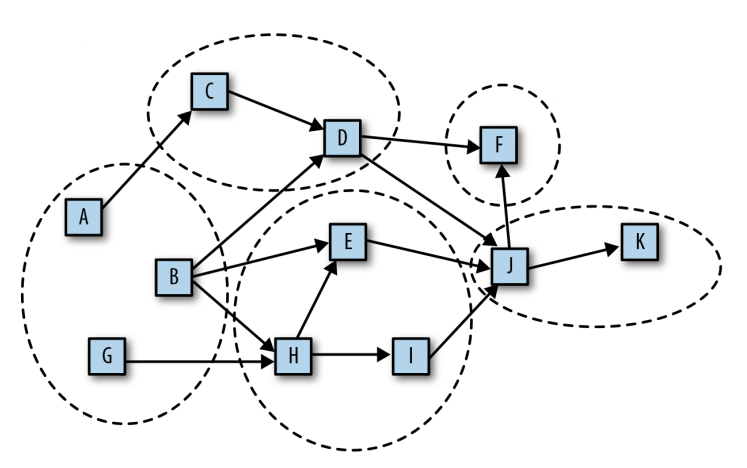
\includegraphics[scale=0.5]{./figure/Cap3/monoFig2.png}
  \caption{Microservicios}\label{figura2}
\end{figure}
Múltiples microservicios pueden ser implementados en el mismo ambiente, aunque no es recomendado, ya que reduce los puntos de falla. En la figura 4 se muestra un ejemplo de una aplicación utilizando la arquitectura de microservicios, en donde se tiene bien definido los dominios de cada servicio. Como se muestra en la \ref{figura2}, se tienen multiples servicios en dominios bien definidos, ademas, de tener bien definido como se comunican entre ellos.

\hypertarget{diseno-basado-en-dominios}{%
\section{Diseño Basado en Dominios}\label{diseno-basado-en-dominios}}

Los fundamentos principales de DDD están basados en la discusión, escuchar, entendimiento, descubrimiento, y valores de negocio, todo esto para poder centralizar el conocimiento. Si eres capaz de entender el negocio en el cual se basará, por lo menos podrá participar en el modelado del software y podrá participar en el proceso de crear el lenguaje ubicuo.

Es un modelo basado en software, el cual esta basado en un dominio de negocio. También considerado como modelo objeto, donde existen objetos, los cuales tienen datos y comportamientos en base al negocio. Crear un modelo del domino es esencial para poder utilizar DDD. Utilizando DDD los modelos del dominio tienden a ser pequeños y enfocados.
Permitir que los expertos del dominio y desarrolladores trabajen en conjunto, lo cual producirá un software que este basado en el negocio.
Centralizar el conocimiento es clave, porque con esto la empresa es capaz de garantizar la comprensión del software.

DDD provee técnicas de desarrollo de software, las cuales se encargan del diseño estratégico y táctico. Diseño estratégico ayuda a entender cuales son las inversiones que se tiene realizar con el software, que tipo de software existe para poder obtener un software rápido y seguro. Diseño táctico ayuda a desarrollar un solo modelo de la solución Newman (2015).

\hypertarget{aspectos-principales-de-ddd}{%
\subsection{Aspectos principales de DDD}\label{aspectos-principales-de-ddd}}
\begin{itemize}
\item
  Acerca a los expertos del dominio y desarrolladores para trabajar en conjunto para reflejar el modelo mental del experto. Al trabajar juntos los expertos del dominio y desarrolladores su principal objetivo es crear un lenguaje ubicuo. Este lenguaje permitirá tener una mejor comunicación y un mayor entendimiento sobre el dominio del negocio.
\item
  DDD aborda las iniciativas estratégicas de la empresa. Aunque DDD incluya técnicas de análisis, esta mas enfocado con la estrategia de dirección de la empresa. Los aspectos técnicos de la estrategia del diseño tiene como objetivo crear bounding system y preocupaciones de negocios.
\item
  Tácticas de diseño permiten a los desarrolladores producir un software que esta correctamente codificado en base a los conocimientos de los expertos del dominio, es escalable, y permite cómputo distribuido.
\end{itemize}
\hypertarget{valores-y-beneficios-de-ddd}{%
\subsection{Valores y beneficios de DDD}\label{valores-y-beneficios-de-ddd}}
\begin{enumerate}
\def\labelenumi{\arabic{enumi}.}
\item
  Organizaciones ganan un modelo útil de su dominio. El objetivo de DDD es invertir todos los esfuerzos en lo que importa más del negocio. Se enfoca en el dominio central (Core domain). Otros modelos existen para dar soporte al dominio central.
\item
  Una definición refinada y precisa del negocio es desarrollado. Cuando el modelo es refinado una y otra vez, se desarrolla un mejor entendimiento el cual se puede utilizar como herramienta de análisis.
\item
  Expertos del dominio contribuyen al diseño del software. Cuando los expertos comparten sus conocimientos entre ellos, permite crear un mejor entendimiento del negocio. Esto, ayuda a el crecimiento de la empresa. Adicionalmente, los desarrolladores comparten un lenguaje ubicuo con los expertos.
\item
  Mejor experiencia de usuario. Usualmente, la retroalimentación del usuario puede transformarse en un mejor reflejo del modelo del dominio. Cuando el software deja mucho al entendimiento del usuario, los usuarios necesitan ser entrenados para poder utilizarlo. En esencia, el usuario solo transfiere su entendimiento del software a datos, los cuales son introducidos al software. Estos datos son guardados. Sí el usuario no entiende exactamente que es lo que necesita introducir, entonces, los resultados no son los correctos.
\item
  Los límites son claros, los cuales son planteados alrededor de los modelos. Los desarrolladores son orientados a utilizar un enfoque de negocio.
\item
  La arquitectura empresarial es mejor organizada. Cuando los límites del contexto son bien definidos y cuidadosamente particionados, todos los equipos tienen un claro entendimiento de donde y porqué las integraciones son necesarias. Los límites son explícitos, y las relaciones entre ellos también.
\item
  Ágil, iterativo, modelado continuo es usado. El objetivo de DDD es refinar el modelo mental de los expertos del dominio a un modelo útil para el negocio.
\item
  Nuevas herramientas, estratégica y tácticas, son utilizadas. El límite contextual da al equipo límites de modelado en donde se crea una solución para un problema especifico en el dominio. Dentro de un límite contextual un lenguaje ubicuo es creado. Este, es utilizado por el equipo y en el modelo del software. Dentro de un límite de modelado pueden utilizar tácticas: Aggregates, Entidades, Objeto Valor, Servicios, Eventos del Dominio, entre otros.
\end{enumerate}
\hypertarget{materiales-y-metodos}{%
\chapter{Materiales y métodos}\label{materiales-y-metodos}}

Intro de Cap

\hypertarget{descripcion-del-area-de-estudio}{%
\section{Descripción del área de estudio}\label{descripcion-del-area-de-estudio}}

\hypertarget{materiales}{%
\section{Materiales}\label{materiales}}

\hypertarget{hardware}{%
\subsection{Hardware}\label{hardware}}

Las herramientas utilizadas fueron las siguientes:
\begin{enumerate}
\def\labelenumi{\arabic{enumi}.}
\tightlist
\item
  Computadora Workstation que cuenta con:
\end{enumerate}
\begin{itemize}
\tightlist
\item
  Procesador \emph{Intel} i7 6800k @4.2GHz de 6 núcleos
\item
  Memoria RAM total de 32 GB @ 2666MHz
\item
  Discos duros:
  \begin{itemize}
  \tightlist
  \item
    \emph{Samsung} 960 EVO 500 GB NVMe SSD
  \item
    SSD 250 GB
  \item
    HDD 1 TB 7200 RPM
  \end{itemize}
\end{itemize}
\begin{enumerate}
\def\labelenumi{\arabic{enumi}.}
\setcounter{enumi}{1}
\tightlist
\item
  Servidor Dell PowerEdge 2950
\end{enumerate}
\begin{itemize}
\tightlist
\item
  2x procesadores Xeon Dual Core
\item
  Memoria RAM total 16 GB
\item
  Discos duros de 200 GB 1500 RPM
\end{itemize}
\begin{enumerate}
\def\labelenumi{\arabic{enumi}.}
\setcounter{enumi}{2}
\tightlist
\item
  Notebook Gateway nv52
\end{enumerate}
\begin{itemize}
\tightlist
\item
  Disco duro de 320GB.
\item
  Procesador AMD Athlon X2 Dual-Core QL-64 2.10Ghz.
\item
  Memoria RAM 4 GB
\end{itemize}
\begin{enumerate}
\def\labelenumi{\arabic{enumi}.}
\setcounter{enumi}{3}
\tightlist
\item
  Notebook ASUS Zenbook
\end{enumerate}
\begin{itemize}
\tightlist
\item
  Procesador \emph{Intel} i5-5200U @ 2.2Ghz
\item
  memoria RAM 8 GB
\item
  Disco duro SSD 250 GB
\end{itemize}
\hypertarget{software}{%
\subsection{Software}\label{software}}

Sistemas operativos utilizados:
\begin{itemize}
\tightlist
\item
  Fedora 26 Workstation
\item
  Fedora 27 Workstation
\item
  Windows 7
\end{itemize}
En cuanto a software se utilizó:
\begin{itemize}
\tightlist
\item
  Python 3
\item
  Flask 0.12.2
\item
  Ansible 2.5.2
\item
  Kubernetes 1.9.8
\item
  Devstack
\item
  Docker 18.03.1-ce, build 9ee9f40
\item
  VIM 8.0.1806
\item
  RStudio 1.1.442
\item
  Kile 4.14.32
\end{itemize}
\hypertarget{metodos}{%
\section{Métodos}\label{metodos}}

\hypertarget{devstack}{%
\subsection{Devstack}\label{devstack}}

\emph{Devstack} Es una serie de scripts y utilidades para poder desplegar una nube \emph{Openstack} (2018b). El proceso de instalación se muestra en el apéndice A.

\hypertarget{configuracion}{%
\subsubsection{Configuración}\label{configuracion}}

Tanto la configuración de usuarios y sus contraseñas son las de fabrica.

\hypertarget{docker}{%
\subsection{Docker}\label{docker}}

\emph{Docker} es una plataforma para la creacion, despliegue de contenedores Mouat (2015).

\hypertarget{modelacion-utilizando-diseno-basado-en-dominios}{%
\chapter{Modelacion utilizando diseño basado en dominios}\label{modelacion-utilizando-diseno-basado-en-dominios}}

\hypertarget{requisitos}{%
\section{Requisitos}\label{requisitos}}
\begin{itemize}
\tightlist
\item
  Permita reconocer el equipo de computo en la red.
\item
  Crear un inventario con el equipo de computo del usuario.
  \begin{itemize}
  \tightlist
  \item
    Permita seleccionar cuales serán las computadoras para la migración.
  \end{itemize}
\item
  Facilitar la creación de respaldos de disco duro
\item
  Migración de los respaldos a la nube
\end{itemize}
Las computadoras del usuario deberán tener lo siguiente:
\begin{itemize}
\tightlist
\item
  \emph{Windows} 7, 8.1 o 10
\item
  \emph{Powershell} 3.0 en adelante
\item
  \emph{NET} 4.0
\item
  \emph{WinRM} deberá ser creado y activado.
\end{itemize}
El modelo siempre debe ser construido teniendo en cuenta las consideraciones de diseño y software. Esto, con el propósito de diseñar un modelo, el cual pueda ser expresado apropiadamente en software.

Una vez analizado los requisitos se encontraron tres subdominios:
\begin{itemize}
\tightlist
\item
  Inventario
\item
  Migración
\item
  Orquestación Vernon (2013)
\end{itemize}
figura pagina 55 de implementacion
\begin{figure}[h!]
  \centering
  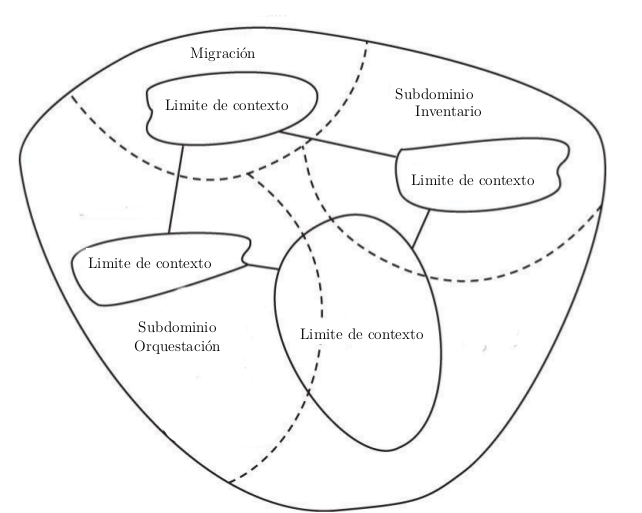
\includegraphics[scale=0.5]{./figure/Cap4/plantillaDDD.png}
  \caption{Modelado del dominio}\label{DDDplantilla}
\end{figure}
Cada uno de estos se explicará a continuación.

\hypertarget{subdominio-inventario}{%
\subsection{Subdominio Inventario}\label{subdominio-inventario}}

\hypertarget{conclusion}{%
\chapter*{Conclusion}\label{conclusion}}
\addcontentsline{toc}{chapter}{Conclusion}

\hypertarget{conclusion-1}{%
\chapter*{Conclusion}\label{conclusion-1}}
\addcontentsline{toc}{chapter}{Conclusion}

\hypertarget{conclusion-2}{%
\chapter*{Conclusion}\label{conclusion-2}}
\addcontentsline{toc}{chapter}{Conclusion}

\appendix

\hypertarget{the-first-appendix}{%
\chapter{The First Appendix}\label{the-first-appendix}}

This first appendix includes all of the R chunks of code that were hidden throughout the document (using the \texttt{include\ =\ FALSE} chunk tag) to help with readibility and/or setup.

\textbf{In the main Rmd file}
\begin{Shaded}
\begin{Highlighting}[]
\CommentTok{# This chunk ensures that the thesisdown package is}
\CommentTok{# installed and loaded. This thesisdown package includes}
\CommentTok{# the template files for the thesis.}
\ControlFlowTok{if}\NormalTok{(}\OperatorTok{!}\KeywordTok{require}\NormalTok{(devtools))}
  \KeywordTok{install.packages}\NormalTok{(}\StringTok{"devtools"}\NormalTok{, }\DataTypeTok{repos =} \StringTok{"http://cran.rstudio.com"}\NormalTok{)}
\ControlFlowTok{if}\NormalTok{(}\OperatorTok{!}\KeywordTok{require}\NormalTok{(thesisdown))}
\NormalTok{  devtools}\OperatorTok{::}\KeywordTok{install_github}\NormalTok{(}\StringTok{"ismayc/thesisdown"}\NormalTok{)}
\KeywordTok{library}\NormalTok{(thesisdown)}
\end{Highlighting}
\end{Shaded}
\textbf{In Chapter \ref{ref-labels}:}

\hypertarget{the-second-appendix-for-fun}{%
\chapter{The Second Appendix, for Fun}\label{the-second-appendix-for-fun}}

\backmatter

\hypertarget{references}{%
\chapter*{References}\label{references}}
\addcontentsline{toc}{chapter}{References}

\markboth{References}{References}

\noindent

\setlength{\parindent}{-0.20in}
\setlength{\leftskip}{0.20in}
\setlength{\parskip}{8pt}

\hypertarget{refs}{}
\leavevmode\hypertarget{ref-Cap3_2_mT}{}%
Ali, I., \& Meghanathan, N. (2011). Virtual machines and networks-installation, performance study, advantages and virtualization options. \emph{arXiv Preprint arXiv:1105.0061}.

\leavevmode\hypertarget{ref-Cap1_4_PdP}{}%
Corp, R. (2011). \emph{R\&M data center handbook} (p. 5). Reichle \& De-Massari AG.

\leavevmode\hypertarget{ref-Cap1_2_PdP}{}%
Delforge, P. (2014). America's data centers are wasting huge amounts of energy. WSP Environment \& Energy, LLC Natural Resources Defense Council. Retrieved from https://www.nrdc.org/sites/default/files/data-center-efficiency-assessment-IB.pdf.

\leavevmode\hypertarget{ref-Cap1_3_PdP}{}%
Dell. (2015). Shipping and delivery. Retrieved from \url{http://www.dell.com/support/Contents/mx/en/mxdhs1/article/eSupport-Order-Support/shipping-and-delivery?~ck=mn}

\leavevmode\hypertarget{ref-Cap3_5_mT}{}%
Foundation, T. A. S. (2017). Apache cloudstack. Retrieved from \url{https://cloudstack.apache.org/}

\leavevmode\hypertarget{ref-Cap1_Hospital}{}%
Frimley. (2018). \emph{Vmware.com}. Retrieved from \url{https://www.vmware.com/content/dam/digitalmarketing/vmware/en/pdf/casestudy/customers/vmware-frimley-park-hospital-13q2-en-case-study.pdf}

\leavevmode\hypertarget{ref-Cap3_8mT}{}%
Geerling, J. (2015). \emph{Ansible for devops: Server and configuration management for humans}. LeanPub.

\leavevmode\hypertarget{ref-Cap1_5_PdP}{}%
Geng, H. (2014). \emph{Data center handbook}. John Wiley \& Sons.

\leavevmode\hypertarget{ref-ibmcloud}{}%
IBM. (2018). Learn what is cloud computing? Retrieved from \url{https://www.ibm.com/cloud/learn/what-is-cloud-computing}

\leavevmode\hypertarget{ref-Cap3_1_mT}{}%
Kusnetzky, D. (2011). \emph{Virtualization: A manager's guide}. " O'Reilly Media, Inc.".

\leavevmode\hypertarget{ref-Cap3_3_mT}{}%
Mell, P., Grance, T., \& others. (2011). The nist definition of cloud computing.

\leavevmode\hypertarget{ref-Cap4_Docker}{}%
Mouat, A. (2015). \emph{Using docker: Developing and deploying software with containers}. " O'Reilly Media, Inc.".

\leavevmode\hypertarget{ref-Cap3_Microservicios}{}%
Newman, S. (2015). \emph{Building microservices: Designing fine-grained systems}. " O'Reilly Media, Inc.".

\leavevmode\hypertarget{ref-Cap3_4_mT}{}%
Openstack. (2015). Software. Retrieved from \url{ttps://www.openstack.org/software/}

\leavevmode\hypertarget{ref-Cap1_ACMInroads}{}%
Pinkelman, J. (1993). Computing changes: An industry perspective. \emph{ACM Inroads}, \emph{4}(4), 39--42.

\leavevmode\hypertarget{ref-Cap3_ArtOfLinux}{}%
Raymond, E. S. (2003). \emph{The art of unix programming}. Addison-Wesley Professional.

\leavevmode\hypertarget{ref-Cap3_6_mT}{}%
Vcloud suite. (2018). \emph{VMWare}. Retrieved from \url{https://www.vmware.com/products/vcloud-suite.html}

\leavevmode\hypertarget{ref-Cap4_ImplementingPlantillaDibujo}{}%
Vernon, V. (2013). \emph{Implementing domain-driven design} (p. 55). Addison-Wesley.

\leavevmode\hypertarget{ref-Cap1_1_PdP}{}%
Whitney, J., \& Kennedy, J. (2012). The carbon emissions of server computing for small-to medium-sized organization. WSP Environment \& Energy, LLC Natural Resources Defense Council. Retrieved from http://www. wspenvironmental. com/media/docs/ourlocations/usa/NRDC-WSP\_Cloud\_Computing. pdf.

\leavevmode\hypertarget{ref-Cap3_7mT}{}%
Wittig, M., \& Wittig, A. (2016). \emph{Amazon web services in action}. Manning.

\leavevmode\hypertarget{ref-Cap1_WebBased}{}%
Zou, Y., \& Kontogiannis, K. (2000). Web-based specification and integration of legacy services. In \emph{Proceedings of the 2000 conference of the centre for advanced studies on collaborative research} (p. 17). IBM Press.

\leavevmode\hypertarget{ref-Cap3_Puppet}{}%
(2017a). \emph{Puppetlabs}. Retrieved from \url{https://www.puppetlabs.com}

\leavevmode\hypertarget{ref-Cap3_ansible}{}%
(2017b). \emph{Red Hat Ansible DevOps made simple}. Retrieved from \url{https://www.ansible.com}

\leavevmode\hypertarget{ref-Cap3_9mT}{}%
(2018a). \emph{Chef}. Retrieved from \url{https://www.chef.io/chef/}

\leavevmode\hypertarget{ref-Cap4_devstack}{}%
(2018b). \emph{Devstack}. Retrieved from \url{https://docs.openstack.org/devstack/latest/}


% Index?

\end{document}
